%%%%%%%%%%%%%%%%%%%%%%%%%%%%%%%%%%%%%%%%%%%%%%%%%%%%%%%%%%%%%%%%%%%%%%%%%%%%%%%%
%%%%%%%%%%%%%%%%%%%%%%%%%%%%%%%%%%%%%%%%%%%%%%%%%%%%%%%%%%%%%%%%%%%%%%%%%%%%%%%%
\exercice{Analyse de la réponse temporelle d'un SLCI~\moyen}
%%%%%%%%%%%%%%%%%%%%%%%%%%%%%%%%%%%%%%%%%%%%%%%%%%%%%%%%%%%%%%%%%%%%%%%%%%%%%%%%
%%%%%%%%%%%%%%%%%%%%%%%%%%%%%%%%%%%%%%%%%%%%%%%%%%%%%%%%%%%%%%%%%%%%%%%%%%%%%%%%
%-------------------------------------------------------------------------------
\begin{center}
    \tikzsetnextfilename{reponse_2nd_ordre-exercices_corriges-chap_model-ext}
    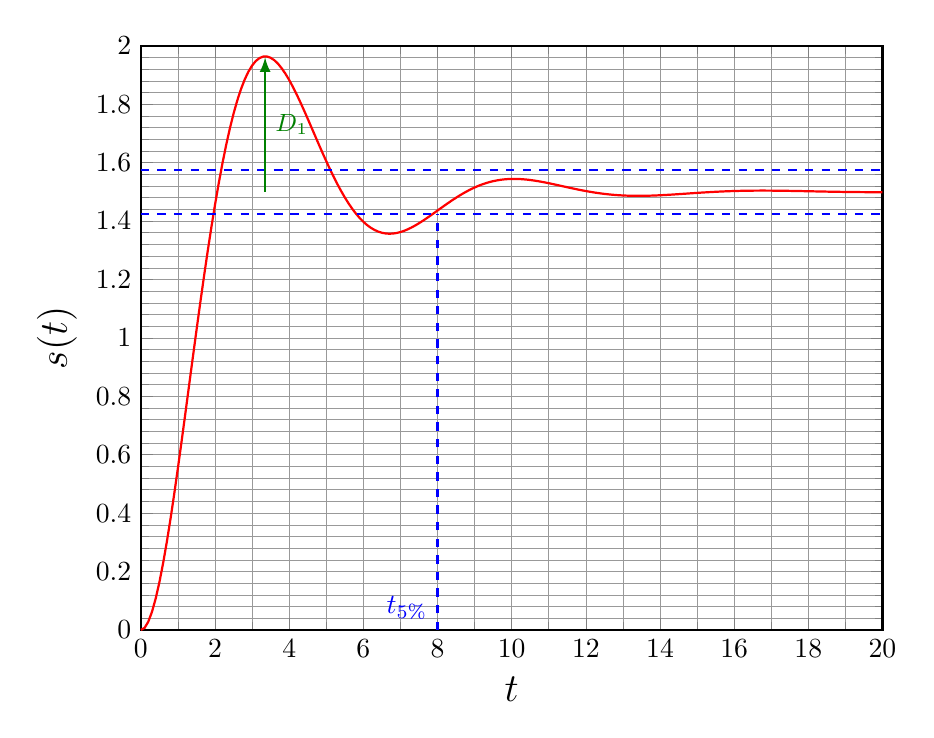
\begin{tikzpicture}
    \pgfmathsetmacro{\kk}{1.5}
    \pgfmathsetmacro{\zz}{0.35}
    \pgfmathsetmacro{\wz}{1.0}
    \pgfmathsetmacro{\aa}{\zz*\wz}
    \pgfmathsetmacro{\bb}{sqrt(1-\zz*\zz)}
    \pgfmathsetmacro{\wwd}{\wz*\bb}
    \pgfmathsetmacro{\mm}{1.0/\bb}
    \pgfmathsetmacro{\pp}{acos(\zz)}
    \begin{axis}
    [
        width=11cm,
        height=9cm,
        legend style={draw=none},
        legend pos=south west,
        axis line style = thick,
        xmin=0,
        xmax=20,
        ymin=0,
        ymax=2,
        xlabel={$t$},
        ylabel={$s(t)$},
        label style={font=\Large},
        minor y tick num=4,
        minor x tick num=1,
        grid=both,
        grid style={line width=.2pt, draw=gray!80},
        major grid style={line width=.2pt,draw=gray!80},
        clip=false,
    ]
    \addplot[thick,color=red,domain=0:20,samples=201]
    {\kk*(1-\mm*exp(-\aa*x)*sin(deg(x)*\wwd+acos(\zz)};%+deg(\pp)))};
    \addplot[dashed,blue,thick,samples=101,domain=0:20] {1.425};
    \addplot[dashed,blue,thick,samples=101,domain=0:20] {1.575};
    \draw[blue,dashed,thick] (axis cs:8,0) node[above left]{$t_{5\%}$} -- 
                             (axis cs:8,1.425);
    \draw[green!50!black,thick,-latex] (axis cs:3.35,1.5) -- 
             node[right] {\small$D_1$} (axis cs:3.35,1.96);
    \end{axis}
\end{tikzpicture}


\end{center}
%-------------------------------------------------------------------------------
%%%%%%%%%%%%%%%%%%%%%%%%%%%%%%%%%%%%%%%%%%%%%%%%%%%%%%%%%%%%%%%%%%%%%%%%%%%%%%%%
\question{\textbf{Déterminer :}}
%%%%%%%%%%%%%%%%%%%%%%%%%%%%%%%%%%%%%%%%%%%%%%%%%%%%%%%%%%%%%%%%%%%%%%%%%%%%%%%%
%-------------------------------------------------------------------------------
\begin{itemize}
    \item Ordre du système : 2nd ordre 
    \item Gain statique $K$ : $K=1.5$ 
    \item Temps de réponse à 5\% : $t_{5\%}\sim\SI{8}{\second}$ 
    \item Dépassement relatif en \% : $D_1\sim\dfrac{1.96-1.5}{1.5}\sim30\%$ 
\end{itemize}
%-------------------------------------------------------------------------------
%%%%%%%%%%%%%%%%%%%%%%%%%%%%%%%%%%%%%%%%%%%%%%%%%%%%%%%%%%%%%%%%%%%%%%%%%%%%%%%%
\question{\textbf{En déduire l'amortissement $\xi$, la pulsation propre 
$\omega_0$ et écrire la fonction de transfert.}}
%%%%%%%%%%%%%%%%%%%%%%%%%%%%%%%%%%%%%%%%%%%%%%%%%%%%%%%%%%%%%%%%%%%%%%%%%%%%%%%%
\`A partir du dépassement : 
\[
\xi=\dfrac{\ln{D}}{\sqrt{\pi^2+(\ln{D})^2}}\sim0.35 
\]

\`A partir du temps du premier dépassement :
$t_1\sim\SI{3.35}{\second}$

\[
\omega_0=\dfrac{\pi}{t_1\sqrt{1-\xi^2}}\sim\SI{1}{\radian\per\sec} 
\]
%%%%%%%%%%%%%%%%%%%%%%%%%%%%%%%%%%%%%%%%%%%%%%%%%%%%%%%%%%%%%%%%%%%%%%%%%%%%%%%%
\question{\textbf{Calculer les pôles du système et les placer les sur une cartes
des pôles (plan complexe).}}
%%%%%%%%%%%%%%%%%%%%%%%%%%%%%%%%%%%%%%%%%%%%%%%%%%%%%%%%%%%%%%%%%%%%%%%%%%%%%%%%
Les pôles sont complexes conjugués et sont donnés par : 
\[
p_{1,2}=-\xi\omega_0\pm j\omega_0\sqrt{1-\xi^2}
\]
$p_1=-0.35+0.93j$ et $p_2=-0.35-0.93j$
%%%%%%%%%%%%%%%%%%%%%%%%%%%%%%%%%%%%%%%%%%%%%%%%%%%%%%%%%%%%%%%%%%%%%%%%%%%%%%%%
%%%%%%%%%%%%%%%%%%%%%%%%%%%%%%%%%%%%%%%%%%%%%%%%%%%%%%%%%%%%%%%%%%%%%%%%%%%%%%%%
\exercice{Réponse temporelle d'un système du second ordre~\moyen}
%%%%%%%%%%%%%%%%%%%%%%%%%%%%%%%%%%%%%%%%%%%%%%%%%%%%%%%%%%%%%%%%%%%%%%%%%%%%%%%%
%%%%%%%%%%%%%%%%%%%%%%%%%%%%%%%%%%%%%%%%%%%%%%%%%%%%%%%%%%%%%%%%%%%%%%%%%%%%%%%%
%%%%%%%%%%%%%%%%%%%%%%%%%%%%%%%%%%%%%%%%%%%%%%%%%%%%%%%%%%%%%%%%%%%%%%%%%%%%%%%%
\question{\textbf{Déterminer les paramètres du second ordre ($K,\omega_0, \xi$) 
de cette équation différentielle.}}
%%%%%%%%%%%%%%%%%%%%%%%%%%%%%%%%%%%%%%%%%%%%%%%%%%%%%%%%%%%%%%%%%%%%%%%%%%%%%%%%
La forme canonique d'un système du second ordre est donnée par :
\[
\devi{s(t)}{2}+2\xi\omega_0\devi{s(t)}{}+\omega_0^2s(t)=K\omega_0^2e(t)
\]
On détermine alors que :
\[
\begin{cases}
    K\omega_0^2=1\\[1em]
    2\xi\omega_0=3\\[1em]
    \omega_0^2=2
\end{cases}\Rightarrow
\begin{cases}
    K=\dfrac{1}{2}\\[1em]
    \xi=\dfrac{3}{2\sqrt{2}}\\[1em]
    \omega_0=\sqrt{2}
\end{cases}
\]
Puisque $\xi>1$, le système est en régime apériodique.
%%%%%%%%%%%%%%%%%%%%%%%%%%%%%%%%%%%%%%%%%%%%%%%%%%%%%%%%%%%%%%%%%%%%%%%%%%%%%%%%
\question{\textbf{Déterminer la fonction de transfert de ce système.}}
%%%%%%%%%%%%%%%%%%%%%%%%%%%%%%%%%%%%%%%%%%%%%%%%%%%%%%%%%%%%%%%%%%%%%%%%%%%%%%%%
La transformée de Laplace de l'équation différentielle nous donne 
pour des conditions d'Heaviside :
\[
    p^2S(p)+3pS(p)+2S(p)=E(p)
\]
La fonction de transfert que l'on note $H(p)$ est alors donnée par :
\[
H(p)=\dfrac{S(p)}{E(p)}=\dfrac{1}{p^2+3p+2}
\]
Les pôles de la fonction de transfert sont -2 et -1. On peut alors 
écrire $H(p)$ sous la forme :
\[
H(p)=\dfrac{1}{(p+1)(p+2)}
\]
%%%%%%%%%%%%%%%%%%%%%%%%%%%%%%%%%%%%%%%%%%%%%%%%%%%%%%%%%%%%%%%%%%%%%%%%%%%%%%%%
\question{\textbf{Déterminer la réponse indicielle de ce système pour une 
entrée $e(t)=1$ et tracer son allure.}}
%%%%%%%%%%%%%%%%%%%%%%%%%%%%%%%%%%%%%%%%%%%%%%%%%%%%%%%%%%%%%%%%%%%%%%%%%%%%%%%%
La réponse indicielle dans le domaine de Laplace est donnée par une 
entrée $E(p)=\dfrac{1}{p}$, soit :
\[
S(p)=\dfrac{1}{p(p+1)(p+2)}
\]
La transformée inverse (c.f ligne 14 de la table) donne :
\[
s(t)=\dfrac{1}{2}(1-2e^{-t}+e^{-2t})
\]
%-------------------------------------------------------------------------------
\begin{center}
    \tikzsetnextfilename{2nd_ordre-exercices_corriges-chap_model-ext}
    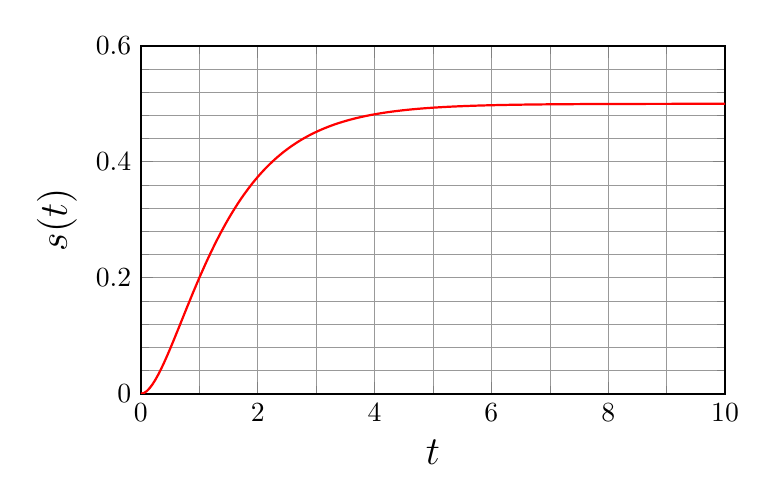
\begin{tikzpicture}
    \begin{axis}[
        width=9cm,
        height=6cm,
        legend style={draw=none},
        legend pos=south west,
        axis line style = thick,
        xmin=0,
        xmax=10,
        ymin=0,
        ymax=0.6,
        xlabel={$t$},
        ylabel={$s(t)$},
        label style={font=\Large},
        minor y tick num=4,
        minor x tick num=1,
        grid=both,
        grid style={line width=.2pt, draw=gray!80},
        major grid style={line width=.2pt,draw=gray!80},
    ]
        \addplot[thick,color=red,domain=0:10,samples=201]
        {0.5*(1-2*exp(-x)+exp(-2*x))};
    \end{axis}
\end{tikzpicture}


\end{center}
%-------------------------------------------------------------------------------
On utilisera les caractéristiques des réponses indicielles du second ordre: 
%-------------------------------------------------------------------------------
\begin{itemize}
    \item pente à l'origine nulle
    \item valeure finale donnée par le théorème de la valeure finale.
\end{itemize}
%-------------------------------------------------------------------------------
%%%%%%%%%%%%%%%%%%%%%%%%%%%%%%%%%%%%%%%%%%%%%%%%%%%%%%%%%%%%%%%%%%%%%%%%%%%%%%%%
%%%%%%%%%%%%%%%%%%%%%%%%%%%%%%%%%%%%%%%%%%%%%%%%%%%%%%%%%%%%%%%%%%%%%%%%%%%%%%%%
\exercice{Modélisation de la chute libre~\moyen}
%%%%%%%%%%%%%%%%%%%%%%%%%%%%%%%%%%%%%%%%%%%%%%%%%%%%%%%%%%%%%%%%%%%%%%%%%%%%%%%%
%%%%%%%%%%%%%%%%%%%%%%%%%%%%%%%%%%%%%%%%%%%%%%%%%%%%%%%%%%%%%%%%%%%%%%%%%%%%%%%%
%%%%%%%%%%%%%%%%%%%%%%%%%%%%%%%%%%%%%%%%%%%%%%%%%%%%%%%%%%%%%%%%%%%%%%%%%%%%%%%%
\question{\textbf{Tracer un schéma représentant le bilan des forces mis en jeu. 
On orientera l'axe de déplacement du haut vers le bas.}}
%%%%%%%%%%%%%%%%%%%%%%%%%%%%%%%%%%%%%%%%%%%%%%%%%%%%%%%%%%%%%%%%%%%%%%%%%%%%%%%%
%-------------------------------------------------------------------------------
\begin{center}
    \tikzsetnextfilename{chute_libre-exercices_corriges-chap_model-ext}
    \begin{tikzpicture}
    \draw[-latex] (0,0) -- (0,-5);
    \draw[-latex,red,thick] (0,-1.5)   --
         node [midway,xshift=1.5em] {$\vect{P}$} (0,-3.5);
    \draw[-latex,green,thick] (0,-1.5) --
         node [midway,xshift=1.5em] {$-k\vect{v}$} (0,-0.5);
    \draw[fill=black] (0,-1.5) circle (3pt) node [xshift=-1.5em] {$m$};
    \node[] at (5,-2.5) {$\vect{P}-k\vect{v}=m\vect{a}$};
\end{tikzpicture}

\end{center}
%-------------------------------------------------------------------------------
%%%%%%%%%%%%%%%%%%%%%%%%%%%%%%%%%%%%%%%%%%%%%%%%%%%%%%%%%%%%%%%%%%%%%%%%%%%%%%%%
\question{\textbf{Déterminer quel système SLCI pourrait être envisagé. 
Quel serait l'entrée et la sortie ?}}
%%%%%%%%%%%%%%%%%%%%%%%%%%%%%%%%%%%%%%%%%%%%%%%%%%%%%%%%%%%%%%%%%%%%%%%%%%%%%%%%
Projetons sur $x$ le bilan des forces. Nous obtenons l'équation différentielle 
suivante :
\[
mg-kv=m\devi{v}{}
\]
ou encore
\[
\dfrac{m}{k}\devi{v}{}+v=\dfrac{m}{k}g
\]
Il est possible de voir se problème comme un système représenté 
par le bloc suivant :
%-------------------------------------------------------------------------------
\begin{center}
    \tikzsetnextfilename{sb_chute_libre-exercices_corriges-chap_model-ext}
    \begin{tikzpicture}
    \sbEntree{E1}
    \sbBloc[3]{B1}{\Large$\Sigma_2$}{E1}
    \sbRelier[\textcolor{red}{$gu(t)$}]{E1}{B1}
    \sbSortie[3]{S1}{B1}
    \sbRelier[\textcolor{blue}{$v(t)$}]{B1}{S1}
\end{tikzpicture}

\end{center}
%-------------------------------------------------------------------------------
C'est à dire que l'entrée correspond à la constante gravitationnelle auquel 
on multiplie la fonction échelon. L'expérience commence quand
\og on prend en compte la gravité\fg.
La sortie est la vitesse que l'on cherche à déterminer.
%%%%%%%%%%%%%%%%%%%%%%%%%%%%%%%%%%%%%%%%%%%%%%%%%%%%%%%%%%%%%%%%%%%%%%%%%%%%%%%%
\question{\textbf{Déterminer l'équation différentielle régissant le système. 
Quels sont son ordre et sa classe ? Quels sont les paramètres de sa forme 
canonique?}}
%%%%%%%%%%%%%%%%%%%%%%%%%%%%%%%%%%%%%%%%%%%%%%%%%%%%%%%%%%%%%%%%%%%%%%%%%%%%%%%%
\[
\dfrac{m}{k}\devi{v}{}+v=\dfrac{m}{k}g
\]
Le système est d'ordre 1 et de classe 0. Les paramètres de la forme canonique 
sont $K=\dfrac{m}{k}$ et $\tau=\dfrac{m}{k}$. Notons qu'il n'y a pas toujours 
égalité de ces deux paramètres.
%%%%%%%%%%%%%%%%%%%%%%%%%%%%%%%%%%%%%%%%%%%%%%%%%%%%%%%%%%%%%%%%%%%%%%%%%%%%%%%%
\question{\textbf{Déterminer la forme de la sortie à partir de la réponse 
temporelle de la forme canonique de ce système. Tracer sa solution.}}
%%%%%%%%%%%%%%%%%%%%%%%%%%%%%%%%%%%%%%%%%%%%%%%%%%%%%%%%%%%%%%%%%%%%%%%%%%%%%%%%
La solution est simplement donnée par la réponse indicielle d'un système du 
premier ordre que nous avons déterminé dans ce chapitre (c.f \cref{eq-1er_ind}),
pour laquelle, $K=\dfrac{m}{k}$, $\tau=\dfrac{m}{k}$ et $E_0=g$.

Soit alors, en prenant $v(0)=0$ :
\[
v(t)=\dfrac{mg}{k}\left(1-e^{-\dfrac{kt}{m}}\right).
\]
La vitesse maximale (c'est à dire la valeur finale de la réponse du SLCI) 
est donc $\dfrac{mg}{k}$ ($KE_0$).
%%%%%%%%%%%%%%%%%%%%%%%%%%%%%%%%%%%%%%%%%%%%%%%%%%%%%%%%%%%%%%%%%%%%%%%%%%%%%%%%
%%%%%%%%%%%%%%%%%%%%%%%%%%%%%%%%%%%%%%%%%%%%%%%%%%%%%%%%%%%%%%%%%%%%%%%%%%%%%%%%
\exercice{\'Etude des systèmes du 1er ordre~\facile}
%%%%%%%%%%%%%%%%%%%%%%%%%%%%%%%%%%%%%%%%%%%%%%%%%%%%%%%%%%%%%%%%%%%%%%%%%%%%%%%%
%%%%%%%%%%%%%%%%%%%%%%%%%%%%%%%%%%%%%%%%%%%%%%%%%%%%%%%%%%%%%%%%%%%%%%%%%%%%%%%%
%%%%%%%%%%%%%%%%%%%%%%%%%%%%%%%%%%%%%%%%%%%%%%%%%%%%%%%%%%%%%%%%%%%%%%%%%%%%%%%%
\question{\textbf{Carte des pôles et zéros. Réponse indicielle.}}
%%%%%%%%%%%%%%%%%%%%%%%%%%%%%%%%%%%%%%%%%%%%%%%%%%%%%%%%%%%%%%%%%%%%%%%%%%%%%%%%
%-------------------------------------------------------------------------------
\begin{itemize}
    \item[(a)] placer son pôle dans la carte des pôles.
    \item[(b)] donner l'allure de la réponse indicielle et estimer le temps
               de réponse à 5\%.
\end{itemize}
%-------------------------------------------------------------------------------
%%%%%%%%%%%%%%%%%%%%%%%%%%%%%%%%%%%%%%%%%%%%%%%%%%%%%%%%%%%%%%%%%%%%%%%%%%%%%%%%
%-------------------------------------------------------------------------------
\begin{center}
    \tikzsetnextfilename{carte_poles-exercices_corriges-chap_model-ext}
    \begin{tikzpicture}[scale=1.2]
    \carte[l]
    \dpole{-1}{0}{1}[blue][below]
    \dpole{-0.5}{0}{2}[blue][below]
    \dpole{-1}{0}{3}[blue][above]
    \dpole{-2}{0}{4}[blue][below]
\end{tikzpicture}

    \tikzsetnextfilename{1er_ordre-exercices_corriges-chap_model-ext}
    \begin{tikzpicture}
    \begin{axis}[
        width=8cm,
        height=6cm,
        legend style={draw=none},
        legend pos=outer north east,
        axis line style = thick,
        xmin=0,
        xmax=8,
        ymin=0,
        ymax=2.1,
        xlabel={$t$},
        ylabel={$s(t)$},
        label style={font=\Large},
        minor y tick num=4,
        minor x tick num=1,
        grid=both,
        grid style={line width=.2pt, draw=gray!80},
        major grid style={line width=.2pt,draw=gray!80},
    ]
        \addplot[thick,color=col1,domain=0:8,samples=201]{(1-exp(-x))};
        \addplot[thick,color=col2,domain=0:8,samples=201]{(1-exp(-0.5*x))};
        \addplot[thick,color=col3,domain=0:8,samples=201]{2*(1-exp(-x))};
        \addplot[thick,color=col4,domain=0:8,samples=201]{(1-exp(-2*x))};
        \legend{$S_1$,$S_2$,$S_3$,$S_4$}
\end{axis}
\end{tikzpicture}

\end{center}
%-------------------------------------------------------------------------------
On trace la réponse indicielle pour des valeurs de $K=1$ et $T=1$.
Le temps de réponse à 5\% de chacun des systèmes est :
%-------------------------------------------------------------------------------
\begin{itemize}
    \item $S_1$: $t_{5\%}=3T$
    \item $S_2$: $t_{5\%}=6T$
    \item $S_3$: $t_{5\%}=3T$
    \item $S_4$: $t_{5\%}=\frac{3}{2}T$
\end{itemize}
%-------------------------------------------------------------------------------
%%%%%%%%%%%%%%%%%%%%%%%%%%%%%%%%%%%%%%%%%%%%%%%%%%%%%%%%%%%%%%%%%%%%%%%%%%%%%%%%
\question{\textbf{Comparer les quatres systèmes en termes de rapidité}}
%%%%%%%%%%%%%%%%%%%%%%%%%%%%%%%%%%%%%%%%%%%%%%%%%%%%%%%%%%%%%%%%%%%%%%%%%%%%%%%%
Le système 4 est bien le plus rapide.
%%%%%%%%%%%%%%%%%%%%%%%%%%%%%%%%%%%%%%%%%%%%%%%%%%%%%%%%%%%%%%%%%%%%%%%%%%%%%%%%
%%%%%%%%%%%%%%%%%%%%%%%%%%%%%%%%%%%%%%%%%%%%%%%%%%%%%%%%%%%%%%%%%%%%%%%%%%%%%%%%
\exercice{Caractéristiques de la réponse temporelle d'un système du 
second ordre~\moyen}
%%%%%%%%%%%%%%%%%%%%%%%%%%%%%%%%%%%%%%%%%%%%%%%%%%%%%%%%%%%%%%%%%%%%%%%%%%%%%%%%
%%%%%%%%%%%%%%%%%%%%%%%%%%%%%%%%%%%%%%%%%%%%%%%%%%%%%%%%%%%%%%%%%%%%%%%%%%%%%%%%
%%%%%%%%%%%%%%%%%%%%%%%%%%%%%%%%%%%%%%%%%%%%%%%%%%%%%%%%%%%%%%%%%%%%%%%%%%%%%%%%
\question{
\textbf{Déterminer la fonction de transfert du second ordre donnant lieu 
à une réponse indicielle aux caractéristiques suivantes :}}
%%%%%%%%%%%%%%%%%%%%%%%%%%%%%%%%%%%%%%%%%%%%%%%%%%%%%%%%%%%%%%%%%%%%%%%%%%%%%%%%
%-------------------------------------------------------------------------------
\begin{itemize}
    \item Dépassement de 10\%
    \item Temps de réponse à 5\% de \SI{8}{\milli\second}
    \item Une sortie égale à l'entrée en régime permanent 
\end{itemize}
%-------------------------------------------------------------------------------
Il est possible de déterminer le coefficient d'amortissement $\xi$ et la 
pulsation propre $\omega_0$ à l'aide des abaques correspondant a
ux~\cref{fig-2nd_depassement_2,fig-2nd_temps_reponse} vus précédement.

Notamment, à partir du dépassement, on cherche l'intersection avec la courbe
pour déterminer $\xi$. Ci-dessous, on détermine une valeur de $\xi=0.59$
%-------------------------------------------------------------------------------
\begin{center}
\tikzsetnextfilename{2nd_depassement-exercices_corriges-chap_model-ext}
\begin{tikzpicture}
    \pgfplotsset{signaltmp/.style={signaln,domain=0.01:0.8277,
                              unbounded coords=jump}
                }
    \pgfmathsetmacro{\pi}{3.141592653589793}     % dépassement d4 
    \begin{axis}
    [   xmode=log,
        ymode=log,
        width=0.6\textwidth,
        axis line style = thick,
        xmin=0.01,
        xmax=1,
        ymin=0.01,
        ymax=1.0,
        xlabel={$\xi$},
        ylabel={$D_k$},
        label style={font=\Large},
        grid=both,
        grid style={line width=.4pt, draw=black},
        major grid style={line width=.4pt,draw=black},
    %    legend style={draw=none,font=\normalsize},
    %    legend pos=outer north east,
    %    legend cell align={left},
        label style={font=\Large},
        clip=false
    ] 
    \pgfmathsetmacro{\xig}{0.59} % xi graphique
    \addplot[signaltmp,vtcol1] {exp(-(x*\pi)/(sqrt(1-x*x)))};
    \addplot[signaltmp,domain=0.01:\xig,very thick, dashed,vtcol4] {0.1};
    \draw[very thick, dashed,vtcol4] (axis cs:\xig,0.01) 
     node [below] {\footnotesize$\xi\sim\xig$} -- (axis cs:\xig,0.1);
     \node[vtcol4,above] at (axis cs:0.015,0.1) {\footnotesize 10\%};
    \end{axis}
\end{tikzpicture}


\end{center}
%-------------------------------------------------------------------------------
Par le calcul, il est possible d'établir $\xi$ en inversant la relation
\Cref{eq-depassement} qui devient :
%-------------------------------------------------------------------------------
\begin{align*}
    \xi=\sqrt{\dfrac{(\ln D)^2}{(\ln D)^2+\pi^2}}
\end{align*}
%-------------------------------------------------------------------------------
Ce qui nous donne une valeur théorique de \SI{0.59115} comparable à la valeur
obtenue graphiquement.

À partir de cette valeur $\xi$, nous pouvons lire une valeur du temps de réponse
à 5\% réduit de 5.35.
%-------------------------------------------------------------------------------
\begin{center}
\tikzsetnextfilename{rapidite_tr_2ndordre-exercices_corriges-chap_model-ext}
\begin{tikzpicture}
    \pgfmathsetmacro{\xig}{0.5911}
    \pgfmathsetmacro{\trg}{5.35}
    \begin{axis}
    [   legend style={draw=none,font=\normalsize},
        legend pos=outer north east,
        axis line style = thick,
        width=0.65\textwidth,
        xmin=1e-1,
        xmax=1e1,
        ymin=1e0,
        ymax=1e2,
        xlabel={$\xi$},
        ylabel={$t_{5\%}\cdot\omega_0$},
        label style={font=\Large},
        legend cell align={left},
        xmode=log,
        ymode=log,
        grid=both,
        grid style={line width=.4pt, draw=black},
        major grid style={line width=.4pt,draw=black},
        clip mode=individual,
        clip=true,
    ]%
        \addplot[mark=none,vtb] table {python/tr.tab};

         \draw[vtr,dashed]    (axis cs:\xig,1) node[below] 
{\footnotesize $\sim$0.59} -- (axis cs:\xig,\trg);
         \draw[vtr,dashed]    (axis cs:0.1,\trg) node [left] 
{\footnotesize $\sim$\trg} -- (axis cs:\xig,\trg);
    \end{axis}
\end{tikzpicture}

\end{center}
%-------------------------------------------------------------------------------
Ce qui nous donne une pulsation propre de 
$\omega_0=\dfrac{5.35}{0.008}=\SI{668.75}{\radian\per\second}$
%-------------------------------------------------------------------------------
Avec ces paramètres, il est possible de reproduire la réponse 
%-------------------------------------------------------------------------------
\begin{center}
    \tikzsetnextfilename{2nd-exercices_corriges-chap_model-ext}
    \begin{tikzpicture}
    \begin{axis}
    [   
        ymax=1.3,
        width=0.65\textwidth,
        axis lines=middle,
        axis line style = {-latex,thick},
        axis x line=center,
        axis y line=center,
        xlabel=$t$,
        ylabel=$s(t)$,
    ]
   \addplot[signalb] table[x=t,y=response] {tikz/2nd-exercices_corriges-chap_model.dat};
   \addplot[dashed,domain=0:0.018] {0.95};
   \addplot[dashed,domain=0:0.018] {1.05};
\end{axis}
\end{tikzpicture}

\end{center}
%-------------------------------------------------------------------------------
%%%%%%%%%%%%%%%%%%%%%%%%%%%%%%%%%%%%%%%%%%%%%%%%%%%%%%%%%%%%%%%%%%%%%%%%%%%%%%%%
%%%%%%%%%%%%%%%%%%%%%%%%%%%%%%%%%%%%%%%%%%%%%%%%%%%%%%%%%%%%%%%%%%%%%%%%%%%%%%%%
\exercice{Réponse temporelle d'un système du premier ordre~\moyen}
%%%%%%%%%%%%%%%%%%%%%%%%%%%%%%%%%%%%%%%%%%%%%%%%%%%%%%%%%%%%%%%%%%%%%%%%%%%%%%%%
%%%%%%%%%%%%%%%%%%%%%%%%%%%%%%%%%%%%%%%%%%%%%%%%%%%%%%%%%%%%%%%%%%%%%%%%%%%%%%%%
Un système linéaire est caractérisé par l'équation :
\[
    0.5\devi{s(t)}{}+s(t)=15e(t)
\]
%%%%%%%%%%%%%%%%%%%%%%%%%%%%%%%%%%%%%%%%%%%%%%%%%%%%%%%%%%%%%%%%%%%%%%%%%%%%%%%%
\question{Donner l'expression de la fonction de transfert du système, la classe,
l'ordre, le gain et la constante de temps de ce système.} 
%%%%%%%%%%%%%%%%%%%%%%%%%%%%%%%%%%%%%%%%%%%%%%%%%%%%%%%%%%%%%%%%%%%%%%%%%%%%%%%%
On applique l'entrée suivante :
%-------------------------------------------------------------------------------
\begin{center}
    \tikzsetnextfilename{sollicitation_1er_ordre-exercices-chap_model-ext}
    \begin{tikzpicture}[baseline=0]
   \begin{axis}[
        height=4cm,
        width=6cm,
        axis x line=center,
        axis y line=center,
        xmin=-1,
        xmax=3,
        ymin=-0.5,
        ymax=1.7,
        xlabel={$t$},
        ylabel={$e(t)$},
        xlabel style={below right},
        ylabel style={left},
        yticklabels={5,$x$},
        ytick={0.8,1.2},
        y tick label style={left},
        xticklabels={\SI{0.1}{\second}},
        xtick={1},
        x tick label style={below},
        ]
        \addplot [very thick,col1,domain=-1:0, samples=50]{0.01};
        \addplot [very thick,col1,domain=0:1, samples=50]{1.2};
        \addplot [very thick,col1,domain=1:2.9, samples=50]{0.8};
        \end{axis}
\end{tikzpicture}

\end{center}
%-------------------------------------------------------------------------------
%%%%%%%%%%%%%%%%%%%%%%%%%%%%%%%%%%%%%%%%%%%%%%%%%%%%%%%%%%%%%%%%%%%%%%%%%%%%%%%%
\question{Donner l'expression de $s(t)$ en fonction de $x$}
%%%%%%%%%%%%%%%%%%%%%%%%%%%%%%%%%%%%%%%%%%%%%%%%%%%%%%%%%%%%%%%%%%%%%%%%%%%%%%%%
%%%%%%%%%%%%%%%%%%%%%%%%%%%%%%%%%%%%%%%%%%%%%%%%%%%%%%%%%%%%%%%%%%%%%%%%%%%%%%%%
\question{Trouver $x$ pour qu'à $t=\SI{0.1}{\second}$ la réponse atteigne 
sa valeur finale et ne la quitte pas}
%%%%%%%%%%%%%%%%%%%%%%%%%%%%%%%%%%%%%%%%%%%%%%%%%%%%%%%%%%%%%%%%%%%%%%%%%%%%%%%%
